\subsection*{Část B}
\begin{itemize}
    \item \textbf{Hlavní úkol:}\\
        \begin{figure}[H]
            \centering
            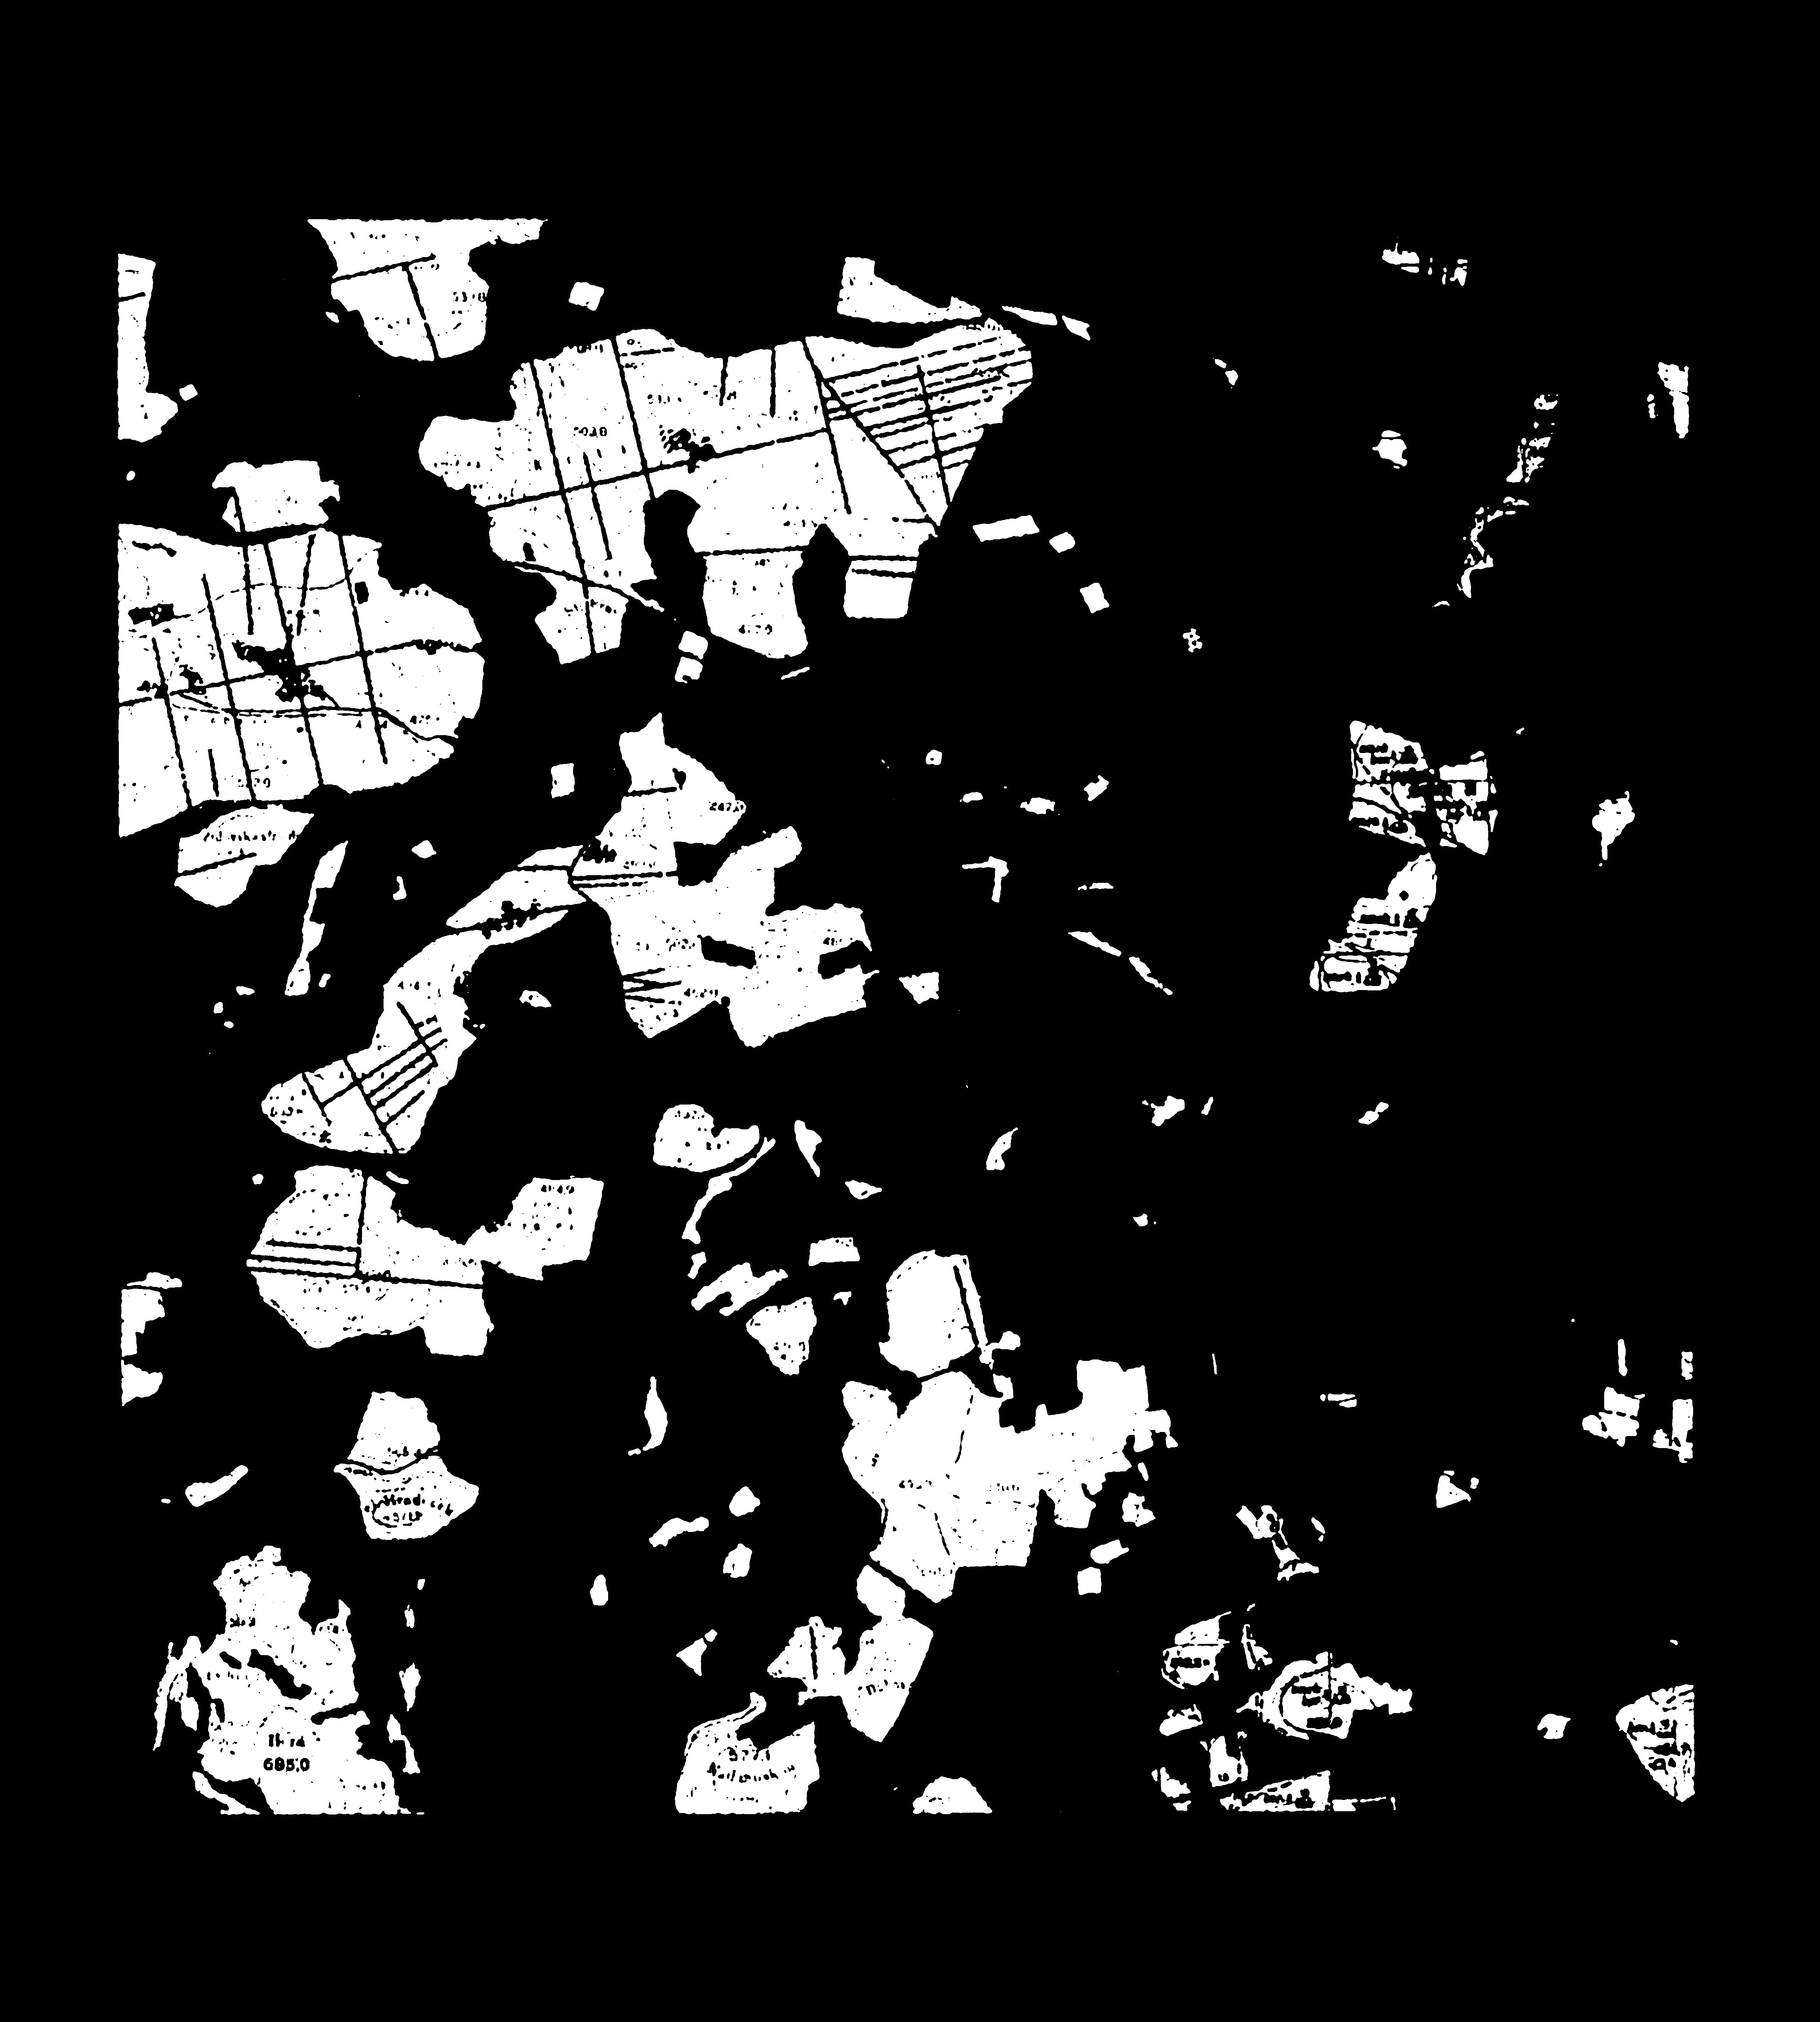
\includegraphics[width=0.9\textwidth]{images/Matlab.jpg}
            \caption{Segmentovaný les z topografické mapy pomocí funkce $k-Means$}
        \end{figure}
        \newpage
    \item \textbf{Bonusový úkol číslo 1:}\\
        \begin{figure}[H]
            \centering
            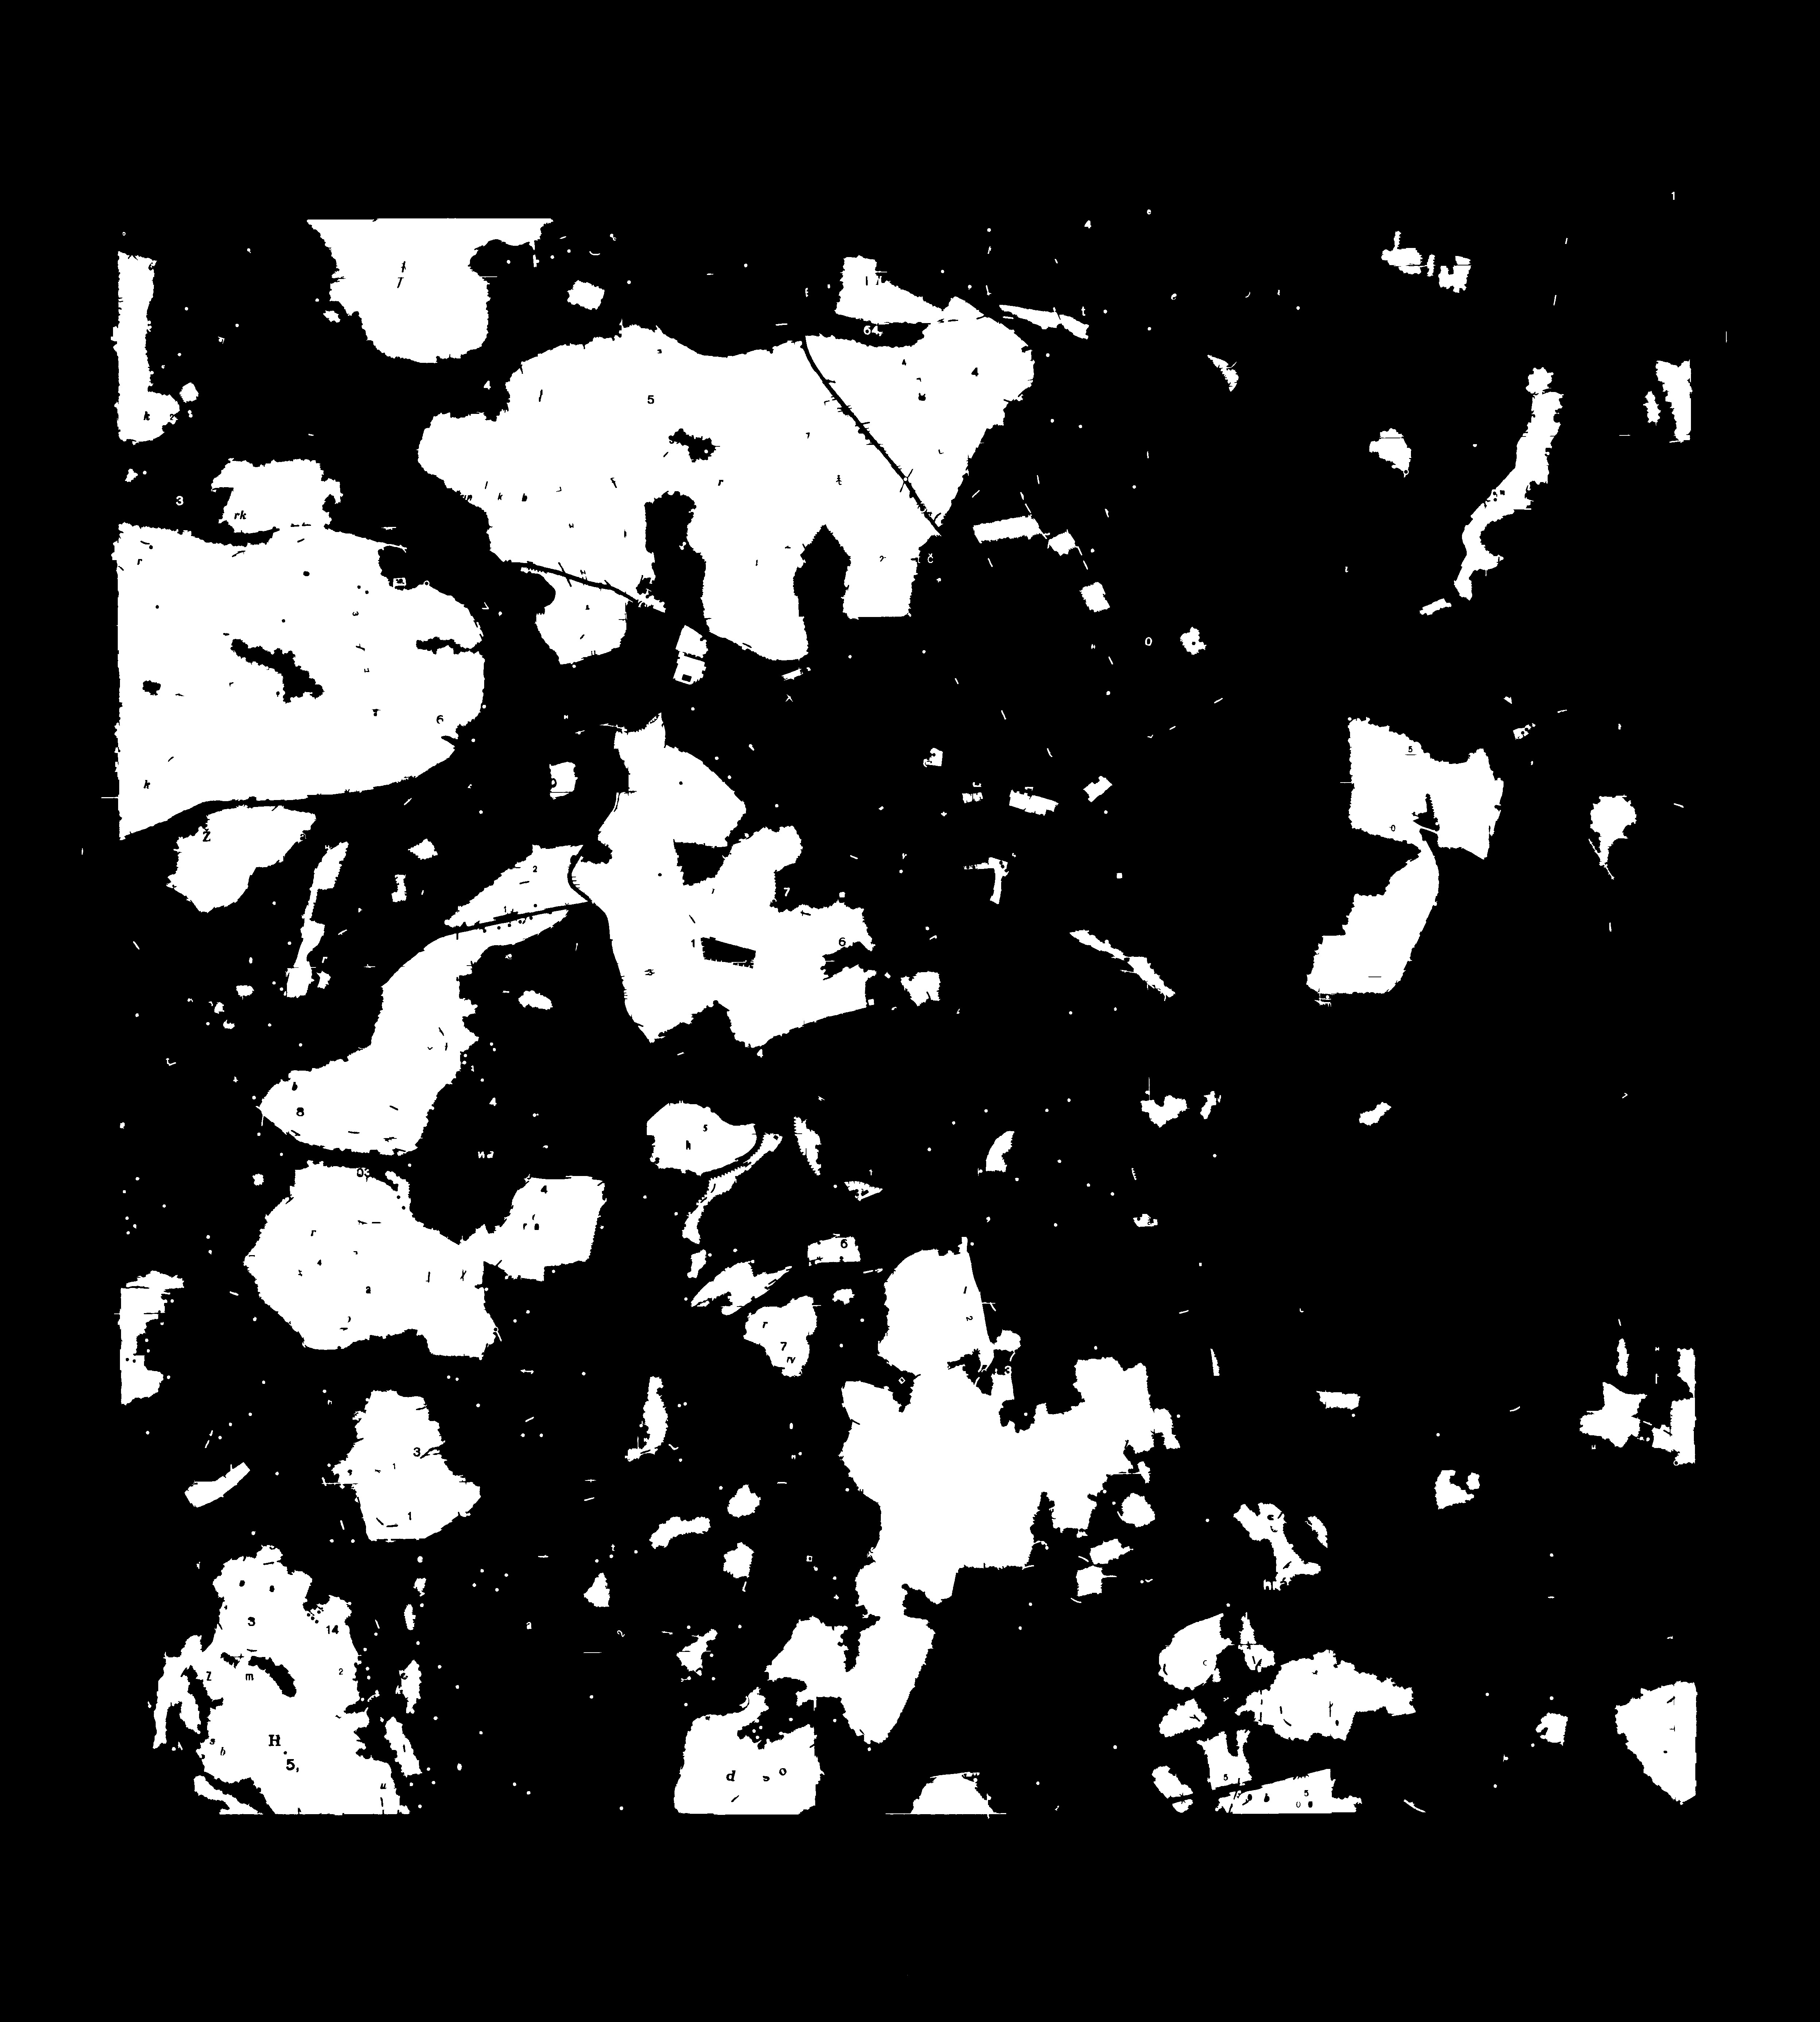
\includegraphics[width=0.9\textwidth]{images/Les_Graph_Cut_BW.jpg}
            \caption{Segmentovaný les z topografické mapy pomocí Graph cut}
        \end{figure}
        \begin{figure}[H]
            \centering
            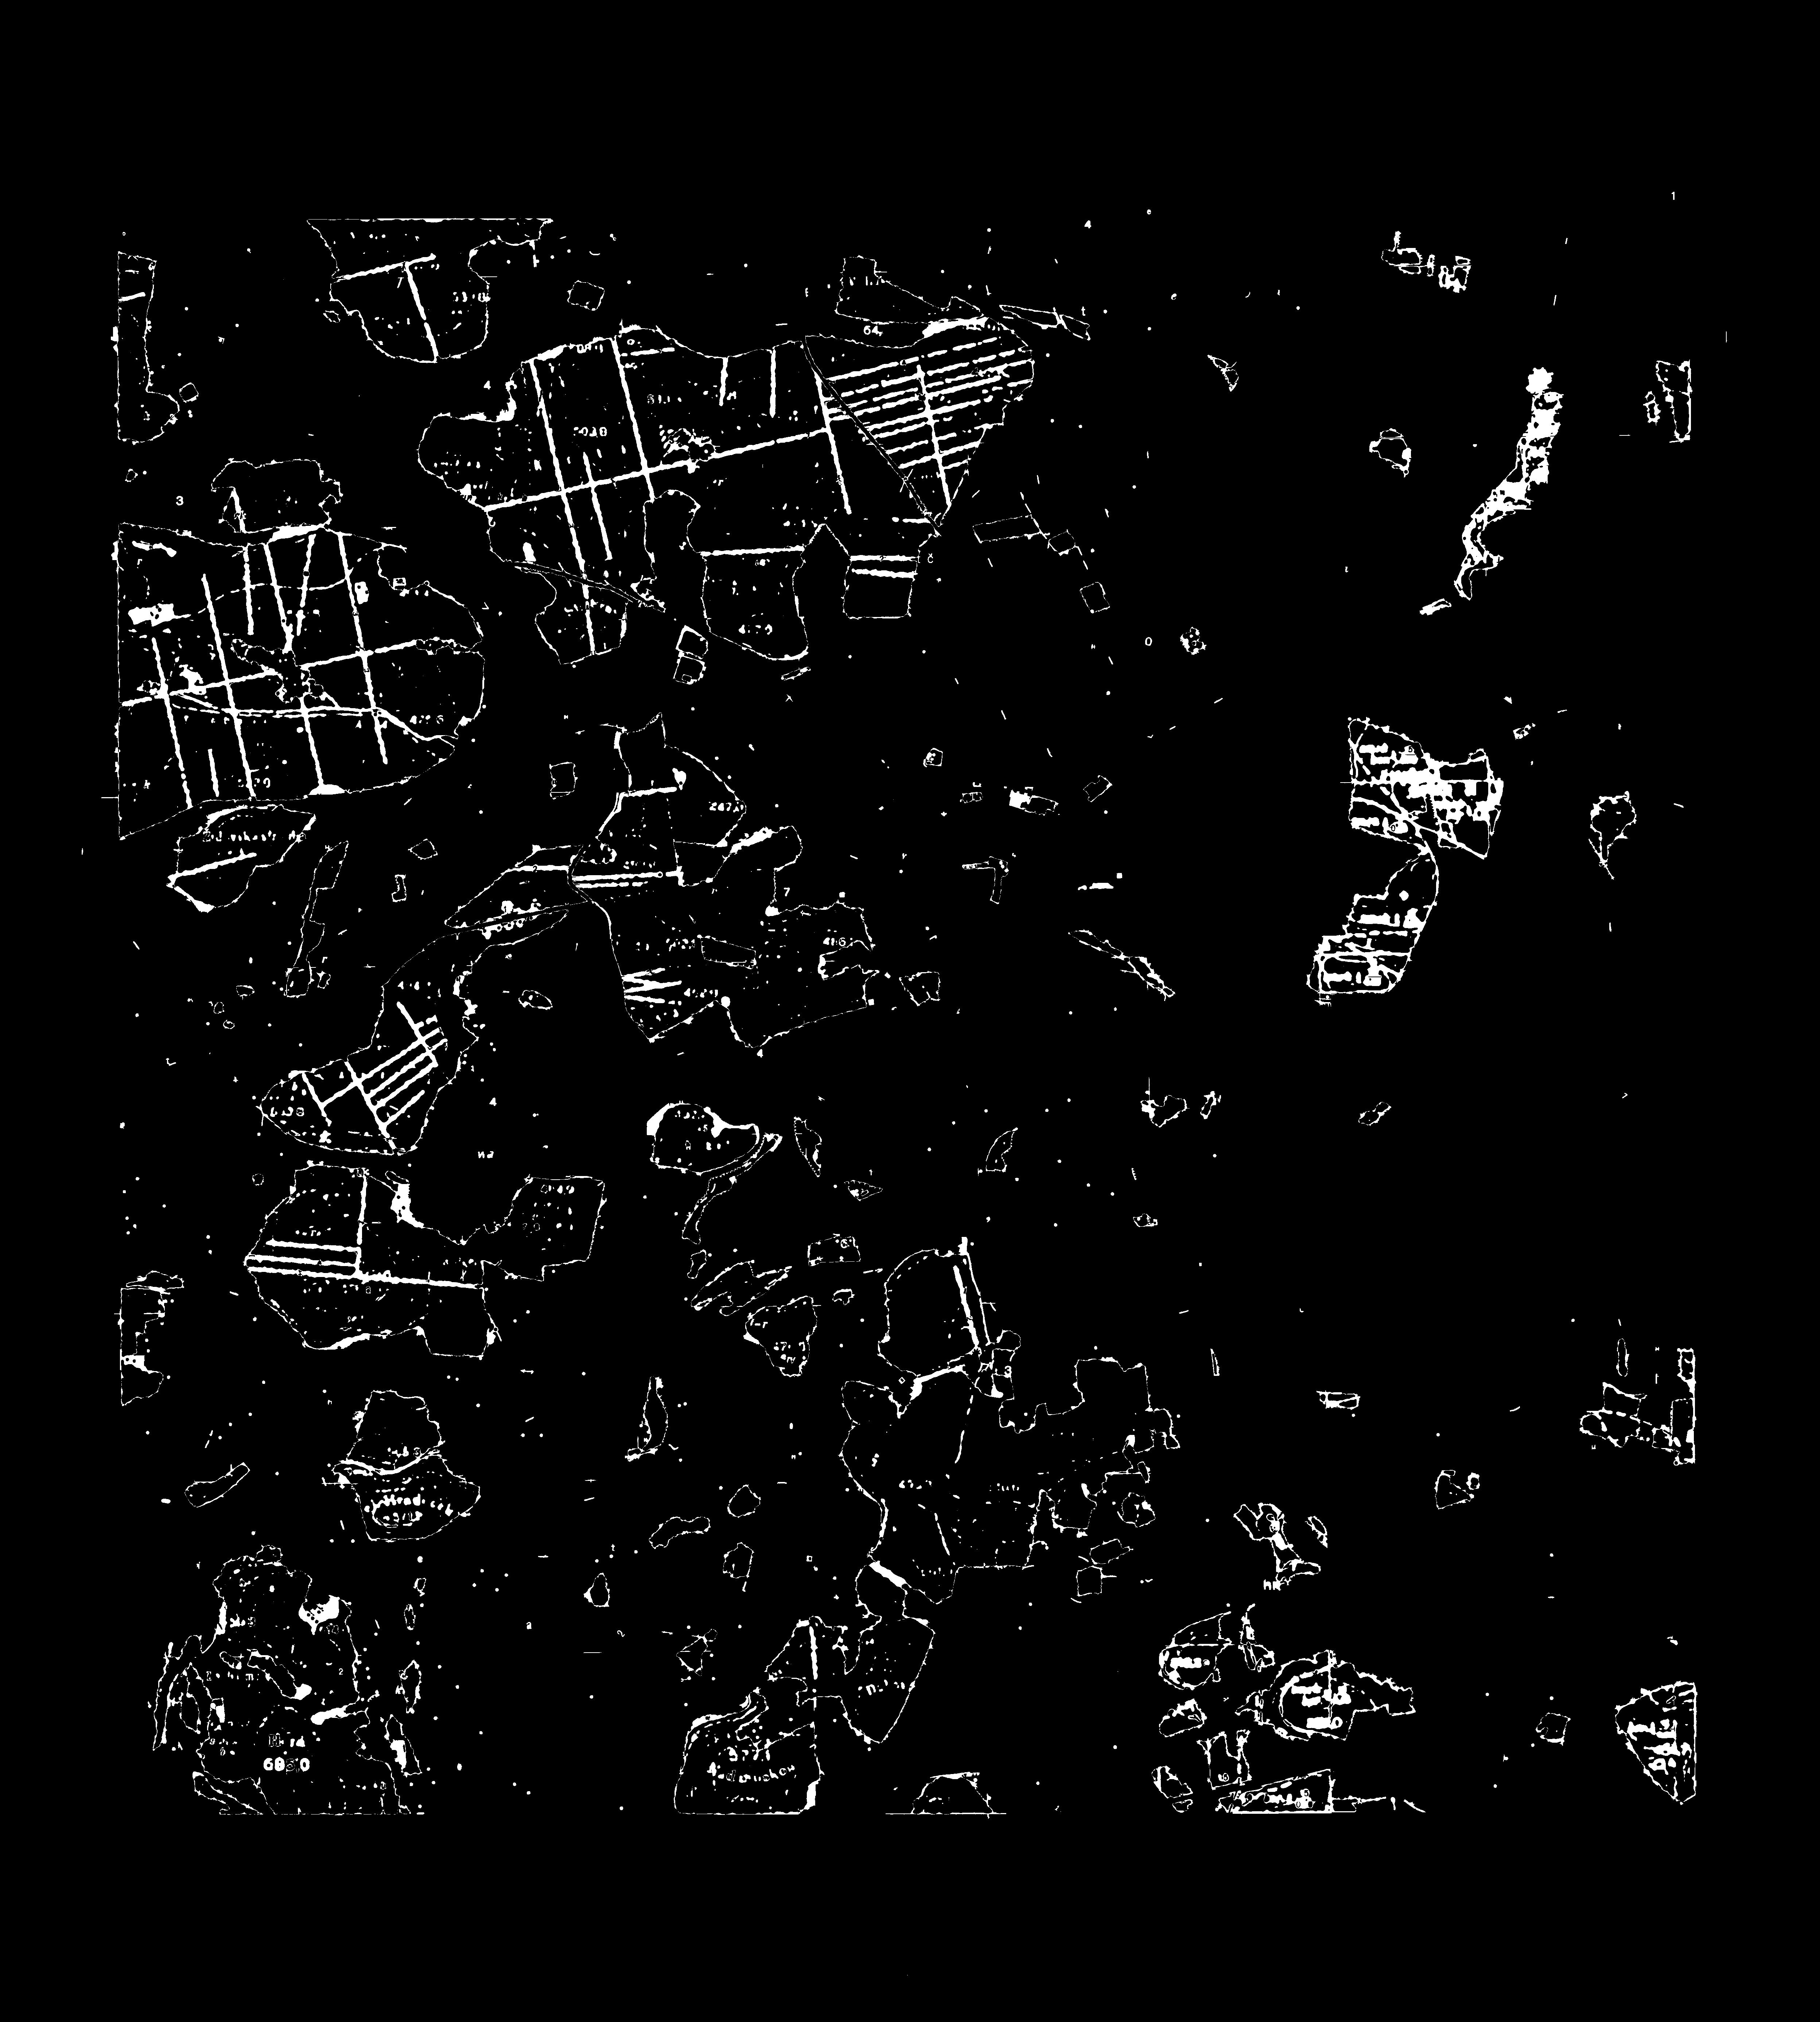
\includegraphics[width=0.9\textwidth]{images/difference.jpg}
            \caption{Rozdíl výsledků}
        \end{figure}
        U porovnání obou výsledků je vidět že filtrací dat přišel výsledek vypočítaný pomocí funkce $k-means$ o kraje segmentovaného lesa. Segmentace pomocí Graph cut si nedokázala poradit s lesními cestami a šumem, který procesem vznikl. Funkce Graph cut si dokázala lépe poradit s problémem, kdy každá část mapy měla různý odstín zelený, způsobený degradací.
    \item \textbf{Bonusový úkol číslo 2:}\\
    Výsledkem je soubor \texttt{Les.gpkg}, který obsahuje polygon segmentovaného lesa v souřadnicovém systému UTM (32633).
\end{itemize}